\chapter{Application Results}
\label{chap:results}

\section{Software Requirements Specification}

\subsection{Overall Description}

PERFIN is a mobile prototype for entering, normalizing, managing and analysing personal-finance data. Chat and media complement forms as input channels. The backend performs every financial calculation, constraint check and data change; LLM, OCR and STT services have no direct PostgreSQL access and are not authoritative numeric sources. FR/NFR identifiers and test traceability follow the requirements-engineering guidance of ISO/IEC/IEEE~29148:2018 \cite{iso29148}.

\begin{table}[H]
  \centering
  \caption{Product context and constraints}
  \label{tab:product-overview}
  \begin{tabularx}{\textwidth}{@{}L{3.5cm}Y@{}}
    \toprule
    \textbf{Item} & \textbf{Description} \\
    \midrule
    User & A general user records and interprets personal-finance data without requiring statistical expertise. \\
    Environment & React Native/Expo on mobile or web, Express API and PostgreSQL; Redis and a worker are configuration-dependent. \\
    System of record & PostgreSQL stores business data; Redis stores only TTL-bound pending, clarification, cache and queue state. \\
    Constraints & The demo uses \code{default_user}, has no production authentication/authorization, defaults to VND and has no foreign-exchange conversion. \\
    Dependencies & Gemini is an external language provider; PaddleOCR and PhoWhisper run locally on the backend host. Local-media failure returns a real error, never fabricated data. \\
    Assumption & The user reviews previews; guidance does not replace professional financial advice. \\
    \bottomrule
  \end{tabularx}
\end{table}

\begin{table}[H]
  \centering
  \caption{Actors and concerns}
  \label{tab:actors}
  \begin{tabularx}{\textwidth}{@{}L{3.2cm}Y Y@{}}
    \toprule
    \textbf{Actor} & \textbf{Role} & \textbf{Concern or limitation} \\
    \midrule
    User & Enters, edits, confirms, manages and views reports. & Language/media-derived data must be reviewed before storage. \\
    External/local AI adapters & Gemini returns a typed draft or narration; local media runtimes return OCR text or a transcript. & No adapter executes business operations or writes the database; extracted text is still untrusted. \\
    Background worker & Runs reminders, analysis and file cleanup. & Jobs require user scope, retry and duplicate-effect protection. \\
    Developer administrator & Configures environment, migrations and providers. & Not a business actor of the application. \\
    \bottomrule
  \end{tabularx}
\end{table}

Shared rules are: business amounts must be finite and valid; transaction dates cannot be in the future; wallets and categories belong to the current profile; negative wallet balances are allowed; chat/media operations require preview and confirmation; multi-record updates are atomic; reports exclude soft-deleted transactions by default; and insufficient data yields a warning or \code{null}, never an invented value.

\subsection{Functional Requirements}

\widereportfigure{14-usecase-overview.pdf}{Overall PERFIN use case diagram. Feature details are specified with flow tables instead of twelve separate diagrams.}{fig:usecase-overview}

Figure~\ref{fig:usecase-overview} contains observable actor goals only. Parser, validation, transaction, TTL and retry behaviour belongs in the flow tables or the sequence/flow diagrams in Section~\ref{subsec:detailed-design}.

\begin{longtable}{@{}L{1.5cm}L{5.0cm}L{3.0cm}L{4.5cm}@{}}
  \caption{Functional-requirement catalogue and location of the full specification}
  \label{tab:fr-catalogue}\\
  \toprule
  \textbf{ID} & \textbf{Capability} & \textbf{Priority} & \textbf{Full specification} \\
  \midrule
  \endfirsthead
  \toprule
  \textbf{ID} & \textbf{Capability} & \textbf{Priority} & \textbf{Full specification} \\
  \midrule
  \endhead
  FR-01 & Natural-language transaction entry & Mandatory & Chapter 3, Table~\ref{tab:fr01} \\
  FR-02 & Image and speech transaction entry & Desirable & Chapter 3, Table~\ref{tab:fr02} \\
  FR-03 & Clarification and confirmation & Mandatory & Chapter 3, Table~\ref{tab:fr03} \\
  FR-04 & Classification and correction retrieval & Mandatory & Chapter 3, Table~\ref{tab:fr04} \\
  FR-05 & Financial-data management & Mandatory & Chapter 3, Table~\ref{tab:fr05} \\
  FR-06 & Wallet transfer and special cash flows & Desirable & Appendix, Table~\ref{tab:app-fr06} \\
  FR-07 & Deterministic financial analytics & Mandatory & Chapter 3, Table~\ref{tab:fr07} \\
  FR-08 & Grounded insights and narration & Desirable & Chapter 3, Table~\ref{tab:fr08} \\
  FR-09 & Budget management and forecasting & Mandatory & Chapter 3, Table~\ref{tab:fr09} \\
  FR-10 & Goal planning and what-if scenarios & Mandatory & Chapter 3, Table~\ref{tab:fr10} \\
  FR-11 & Recurring bills and proactive jobs & Desirable & Appendix, Table~\ref{tab:app-fr11} \\
  FR-12 & Export and expired-file cleanup & Optional & Appendix, Table~\ref{tab:app-fr12} \\
  \bottomrule
\end{longtable}

\begin{frtable}{FR-01 --- Enter Transactions from Text}{tab:fr01}
  \textbf{Feature name} & Enter transactions from natural-language text. \frtablerow
  \textbf{ID} & FR-01. \frtablerow
  \textbf{User} & User. \frtablerow
  \textbf{Necessity} & Mandatory. \frtablerow
  \textbf{Classification} & Complex. \frtablerow
  \textbf{Participants and concerns} & The user needs fast entry; the AI Orchestrator returns a typed draft; Transaction Service protects the ledger. \frtablerow
  \textbf{Summary} & Convert one sentence into one or more structured transactions and create a preview before writing. \frtablerow
  \textbf{Relationships} & Includes FR-03 and FR-04; uses FR-05 after confirmation. \frtablerow
  \textbf{Normal flow} & \textbf{Step 1:} User submits text. \textbf{Step 2:} Extract and normalize. \textbf{Step 3:} Validate schema, category and wallet. \textbf{Sub 1:} Build preview. \textbf{Step 4:} User confirms. \textbf{Step 5:} Commit atomically and return the result. \frtablerow
  \textbf{Subflows} & \textbf{Sub 1 --- Preview:} (1) Store a TTL-bound draft; (2) show amount, type, date, category, wallet and warnings. \frtablerow
  \textbf{Alternate flows} & \textbf{Step 2:} Provider failure uses the local parser or returns an error. \textbf{Step 3:} Missing/ambiguous fields invoke FR-03. \textbf{Step 4:} Edit or cancel causes no write. \frtablerow
\end{frtable}

\begin{frtable}{FR-02 --- Enter Transactions from Image or Speech}{tab:fr02}
  \textbf{Feature name} & Enter a transaction from a receipt image or speech. \frtablerow
  \textbf{ID} & FR-02. \frtablerow
  \textbf{User} & User; local media runtime; optional external language adapter. \frtablerow
  \textbf{Necessity} & Desirable. \frtablerow
  \textbf{Classification} & Complex. \frtablerow
  \textbf{Participants and concerns} & The user needs visible raw text; local OCR/STT reports provider and failure; the backend rejects invalid files. \frtablerow
  \textbf{Summary} & Convert image/audio into reviewable text, then reuse FR-01. \frtablerow
  \textbf{Relationships} & Includes FR-01 and FR-03. \frtablerow
  \textbf{Normal flow} & \textbf{Step 1:} Select a valid file. \textbf{Step 2:} Backend invokes OCR or STT. \textbf{Step 3:} Display raw text and provider. \textbf{Sub 1:} User edits/confirms text. \textbf{Step 4:} Continue with FR-01. \frtablerow
  \textbf{Subflows} & \textbf{Sub 1 --- Media review:} (1) edit a voice transcript; (2) for a receipt, select total or individual items when present. \frtablerow
  \textbf{Alternate flows} & Invalid type or size above 10 MB is rejected. A provider that returns no text produces an error and no mock or pending draft. \frtablerow
\end{frtable}

\begin{frtable}{FR-03 --- Clarify and Confirm Pending Transactions}{tab:fr03}
  \textbf{Feature name} & Clarification, preview and pending-transaction confirmation. \frtablerow
  \textbf{ID} & FR-03. \frtablerow
  \textbf{User} & User. \frtablerow
  \textbf{Necessity} & Mandatory. \frtablerow
  \textbf{Classification} & Complex. \frtablerow
  \textbf{Participants and concerns} & The user can edit/cancel; the KV store applies TTL; a preview can be consumed once. \frtablerow
  \textbf{Summary} & Collect missing fields across turns and prevent inferred data from being written. \frtablerow
  \textbf{Relationships} & Used by FR-01, FR-02, FR-09, FR-10 and FR-12. \frtablerow
  \textbf{Normal flow} & Store intent and missing fields; ask for the next field; merge and revalidate; build/edit a preview; atomically claim pending state; call the business service. \frtablerow
  \textbf{Subflows} & \textbf{Preview:} attach a \code{pending_id} with five-minute TTL and update only with a valid payload. \frtablerow
  \textbf{Alternate flows} & Continue asking while fields are missing. Expired, incorrect or claimed IDs cannot write; cancellation clears state. \frtablerow
\end{frtable}

\begin{frtable}{FR-04 --- Classify and Learn from Corrections}{tab:fr04}
  \textbf{Feature name} & Category classification and correction retrieval. \frtablerow
  \textbf{ID} & FR-04. \frtablerow
  \textbf{User} & User. \frtablerow
  \textbf{Necessity} & Mandatory. \frtablerow
  \textbf{Classification} & Complex. \frtablerow
  \textbf{Participants and concerns} & The matcher must be explainable; the user corrects labels; feedback failure must not corrupt a committed transaction. \frtablerow
  \textbf{Summary} & Select a category by exact/alias/fuzzy/LLM methods and reuse confirmed corrections. \frtablerow
  \textbf{Relationships} & Extends FR-01 and may be triggered by an FR-05 category edit. \frtablerow
  \textbf{Normal flow} & Normalize description; load same-profile categories/corrections; rank candidates; apply a strong correction; return category, confidence and match kind; store feedback after confirmation. \frtablerow
  \textbf{Subflows} & Select at most five similar corrections and use them as context or a controlled override. \frtablerow
  \textbf{Alternate flows} & Low score, small margin or conflicting corrections return Other/request a selection. Feedback-write failure is logged only. \frtablerow
\end{frtable}

\begin{frtable}{FR-05 --- Manage Financial Data}{tab:fr05}
  \textbf{Feature name} & Manage transactions, wallets and categories. \frtablerow
  \textbf{ID} & FR-05. \frtablerow
  \textbf{User} & User. \frtablerow
  \textbf{Necessity} & Mandatory. \frtablerow
  \textbf{Classification} & Complex. \frtablerow
  \textbf{Participants and concerns} & The user needs CRUD and restore; services maintain balance and history consistency. \frtablerow
  \textbf{Summary} & Create, view, edit, soft-delete and restore transactions and manage profile-scoped categories/wallets. \frtablerow
  \textbf{Relationships} & Used by FR-01/FR-02 and supplies FR-07--FR-12. \frtablerow
  \textbf{Normal flow} & Select operation; validate payload and ownership; compute balance delta; update transaction and wallet atomically; return record and new balance. \frtablerow
  \textbf{Subflows} & Write the transaction, update the wallet, commit, then invalidate cache best-effort. \frtablerow
  \textbf{Alternate flows} & Out-of-scope IDs or invalid payloads are rejected. A negative balance remains valid. Any pre-commit failure rolls back. \frtablerow
\end{frtable}

\begin{frtable}{FR-07 --- Analyse Financial Data}{tab:fr07}
  \textbf{Feature name} & Trend, anomaly, runway, recurring and correlation analysis. \frtablerow
  \textbf{ID} & FR-07. \frtablerow
  \textbf{User} & User; Background worker. \frtablerow
  \textbf{Necessity} & Mandatory. \frtablerow
  \textbf{Classification} & Complex. \frtablerow
  \textbf{Participants and concerns} & Analytics needs clean data; users need period, sample size and method. \frtablerow
  \textbf{Summary} & Compute deterministic facts over non-deleted data; trend/correlation use completed periods and fixed calendar axes are zero-filled. \frtablerow
  \textbf{Relationships} & Reads FR-05 and supplies FR-08 and FR-11. \frtablerow
  \textbf{Normal flow} & Select analysis and period; query profile data; normalize the calendar axis and check sample count; run the algorithm; return facts with window, method, parameter and warning metadata. \frtablerow
  \textbf{Subflows} & Run OLS, z-score/IQR, runway, recurring or Pearson through one result contract. \frtablerow
  \textbf{Alternate flows} & Sparse data or zero variance returns a degraded result or \code{null}; no causal claim or fabricated transaction. \frtablerow
\end{frtable}

\begin{frtable}{FR-08 --- Generate Grounded Insights}{tab:fr08}
  \textbf{Feature name} & Grounded insight and persona narration. \frtablerow
  \textbf{ID} & FR-08. \frtablerow
  \textbf{User} & User; External AI service. \frtablerow
  \textbf{Necessity} & Desirable. \frtablerow
  \textbf{Classification} & Complex. \frtablerow
  \textbf{Participants and concerns} & The user needs clear explanation; Analytics owns facts; the narrator cannot alter numbers. \frtablerow
  \textbf{Summary} & Explain precomputed facts and return them with the narration for traceability. \frtablerow
  \textbf{Relationships} & Includes FR-07 and may use a persona when consent is enabled. \frtablerow
  \textbf{Normal flow} & Receive a question/report request; generate facts; load a permitted persona; narrate facts; return narration, facts and provider metadata. \frtablerow
  \textbf{Subflows} & Lock numbers/units in the prompt and use a deterministic template when the provider fails. \frtablerow
  \textbf{Alternate flows} & Sparse facts return a warning. A complete numeric-grounding checker remains a design target and is not presented as measured. \frtablerow
\end{frtable}

\begin{frtable}{FR-09 --- Manage and Forecast Budgets}{tab:fr09}
  \textbf{Feature name} & Monthly budgets, recommendations and forecasts. \frtablerow
  \textbf{ID} & FR-09. \frtablerow
  \textbf{User} & User. \frtablerow
  \textbf{Necessity} & Mandatory. \frtablerow
  \textbf{Classification} & Medium. \frtablerow
  \textbf{Participants and concerns} & Users need progress visibility; Budget Engine needs sufficient history and must not apply limits automatically. \frtablerow
  \textbf{Summary} & Compute spent/remaining, forecast month end and propose limits from history or a ratio framework. \frtablerow
  \textbf{Relationships} & Reads FR-05 and may invoke FR-03 from chat. \frtablerow
  \textbf{Normal flow} & Select month; query spending; compute progress and forecast; produce warning/recommendation; confirm before saving a recommendation. \frtablerow
  \textbf{Subflows} & Zero-fill months; compute limits; proportionally shrink raw allocations and reconcile rounding when a group exceeds its cap. \frtablerow
  \textbf{Alternate flows} & Fewer than three history months produce a warning. A non-positive amount or non-expense category is rejected. \frtablerow
\end{frtable}

\begin{frtable}{FR-10 --- Plan Goals and What-if Scenarios}{tab:fr10}
  \textbf{Feature name} & Savings, purchase and debt-payoff goal planning. \frtablerow
  \textbf{ID} & FR-10. \frtablerow
  \textbf{User} & User. \frtablerow
  \textbf{Necessity} & Mandatory. \frtablerow
  \textbf{Classification} & Complex. \frtablerow
  \textbf{Participants and concerns} & The user needs formula-backed progress; Goal Planner must expose infeasible assumptions. \frtablerow
  \textbf{Summary} & Calculate contribution, duration, amortization and what-if plans without modifying the original until confirmation. \frtablerow
  \textbf{Relationships} & Reads FR-05/FR-07 and may use FR-03. \frtablerow
  \textbf{Normal flow} & Enter goal; validate amount/date/rate; compute allocatable cash; run goal-specific formula; return plan and warnings; save after confirmation. \frtablerow
  \textbf{Subflows} & What-if reruns the saving/purchase function with an additional contribution; debt payoff uses monthly simulation. The original plan is unchanged and no scenario is persisted. \frtablerow
  \textbf{Alternate flows} & Invalid inputs request correction. Payment less than or equal to first-month interest warns of negative amortization; zero payment and a 600-month horizon are reported explicitly. Cancel causes no write. \frtablerow
\end{frtable}

\subsection{Non-functional Requirements}

\begin{longtable}{@{}L{1.3cm}L{3.0cm}L{5.8cm}L{3.8cm}@{}}
  \caption{Non-functional requirements and acceptance methods}\label{tab:nfr}\\
  \toprule
  \textbf{ID} & \textbf{Group} & \textbf{Testable requirement} & \textbf{Measurement} \\
  \midrule
  \endfirsthead
  \toprule
  \textbf{ID} & \textbf{Group} & \textbf{Testable requirement} & \textbf{Measurement} \\
  \midrule
  \endhead
  NFR-01 & Recovery & Provider/Redis failure fabricates no data; restore demo service and backup data within three hours after an incident. & Fault injection, restart and restore on a test database. \\
  NFR-02 & Integrity & No partial create, update, delete, restore, transfer or payment; credentials are never transmitted or logged in clear text. & Rollback tests and configuration/log scanning; TLS for network deployment. \\
  NFR-03 & UI & Vietnamese warm terracotta--cream interface, consistent navigation and no overflow at mobile viewports. & Chromium Expo-web smoke on Dashboard, Budget, Report, Chat preview and Goal plan at measured 390$\times$844; runner supports 360$\times$800 and 412$\times$915 reruns. \\
  NFR-04 & Timing & Acknowledge within three seconds; target text p95 $\leq3$ s and media p95 $\leq8$ s in a disclosed environment. & At least 30 runs per flow with provider, hardware, cache and error rate. \\
  NFR-05 & Correctness & Algorithms match expected normal/boundary cases; negative balances are valid; narrator invents no number. & Unit tests, invariants and facts--response checker. \\
  NFR-06 & Privacy & Remove temporary media; use traits only with consent; ID queries include user scope. & Temporary-file, consent and cross-scope tests. \\
  NFR-07 & Worker consistency & Retrying an event/job creates no duplicate payment, message or export. & Repeat fingerprints and count effects. \\
  NFR-08 & Traceability & Analysis includes schema version, timestamp, component value and metadata for unit, window, sample count, method, parameters, warnings and degradation status. & Contract tests and FR--test--artifact matrix. \\
  \bottomrule
\end{longtable}

Recovery, latency, OCR/STT accuracy and complete numeric grounding remain acceptance targets; unmeasured targets are not presented as achieved results.

\subsubsection{Mobile-web UI smoke evidence}

The following captures are generated from the running Expo web build with synthetic
demo data, viewport $390\times844$ CSS pixels and device scale factor 2. They verify
layout and a review-before-write interaction; they are not native-device screenshots
or UAT evidence.

\begin{figure}[p]
  \centering
  \begin{minipage}[t]{0.47\textwidth}
    \centering
    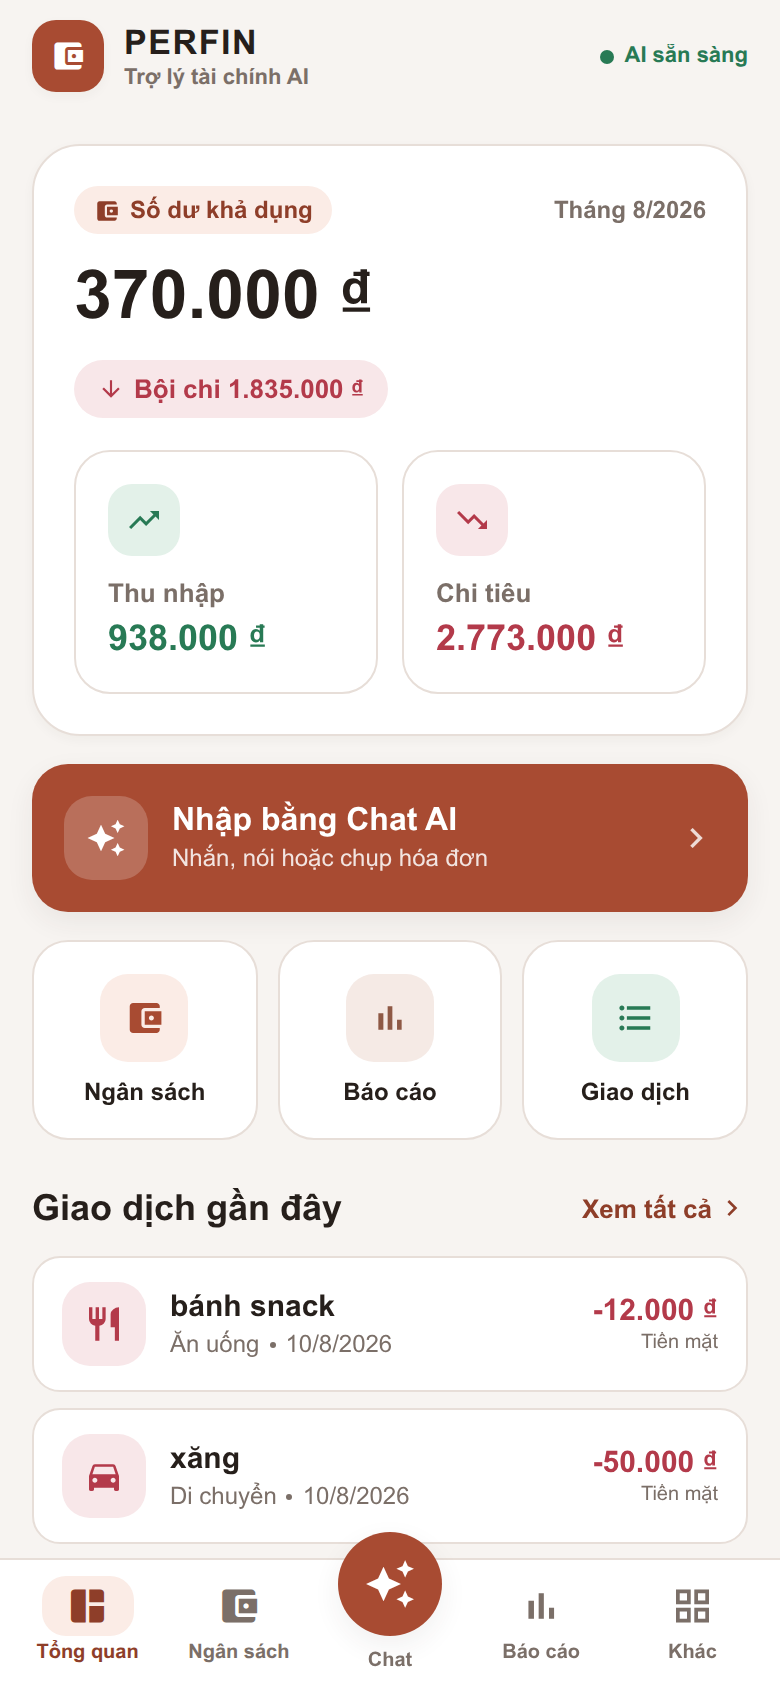
\includegraphics[width=\linewidth,height=0.48\textheight,keepaspectratio]{figures/screenshots/01-dashboard.png}
  \end{minipage}\hfill
  \begin{minipage}[t]{0.47\textwidth}
    \centering
    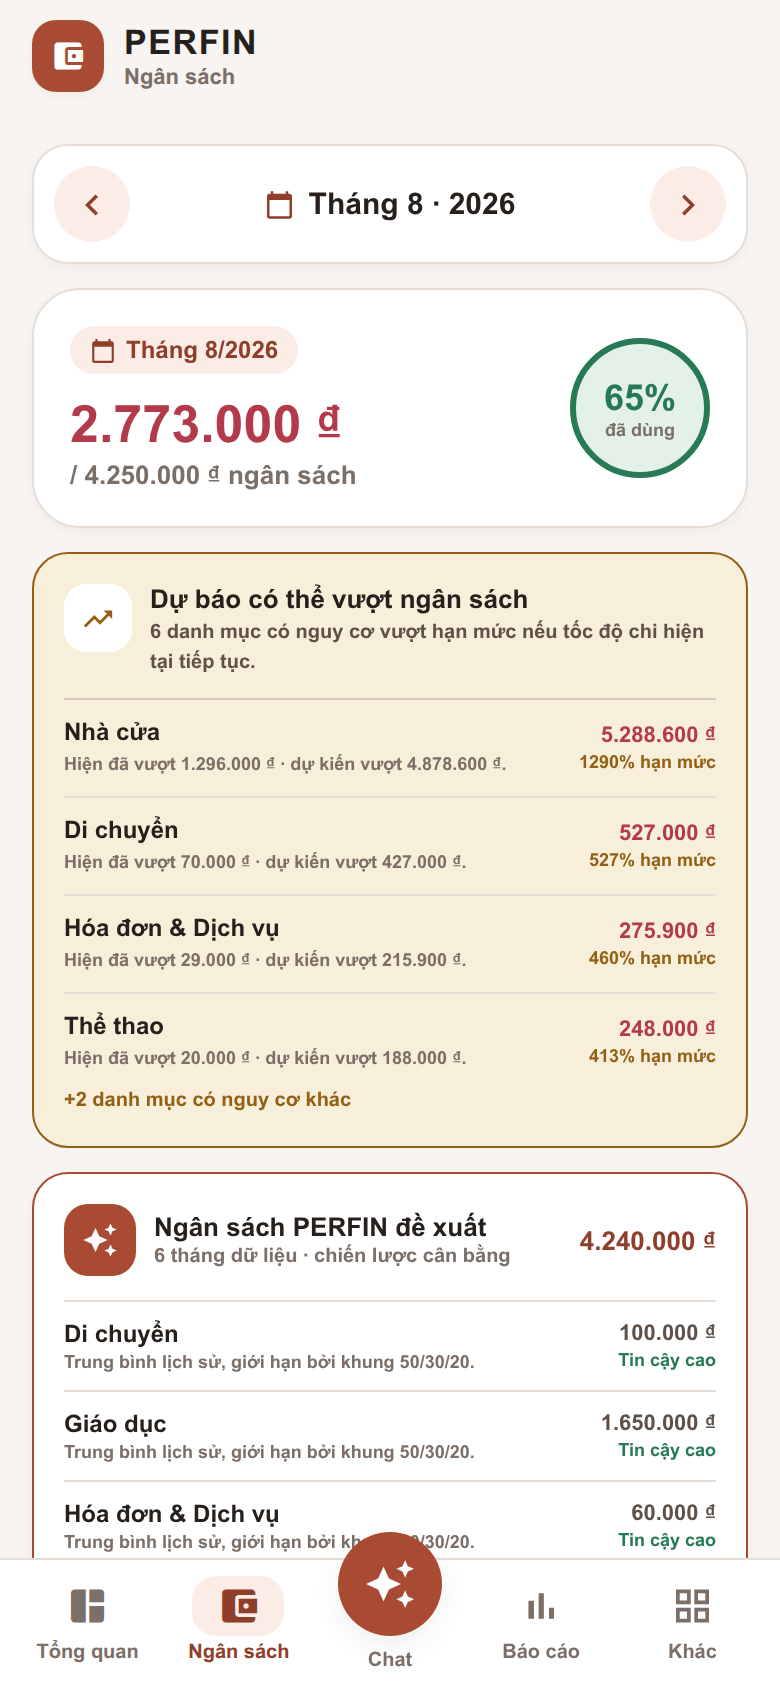
\includegraphics[width=\linewidth,height=0.48\textheight,keepaspectratio]{figures/screenshots/03-budget.png}
  \end{minipage}
  \caption{Expo web mobile viewport: Dashboard and Budget smoke captures (synthetic data; not a physical device).}
  \label{fig:ui-dashboard-budget}
\end{figure}

\begin{figure}[p]
  \centering
  \begin{minipage}[t]{0.47\textwidth}
    \centering
    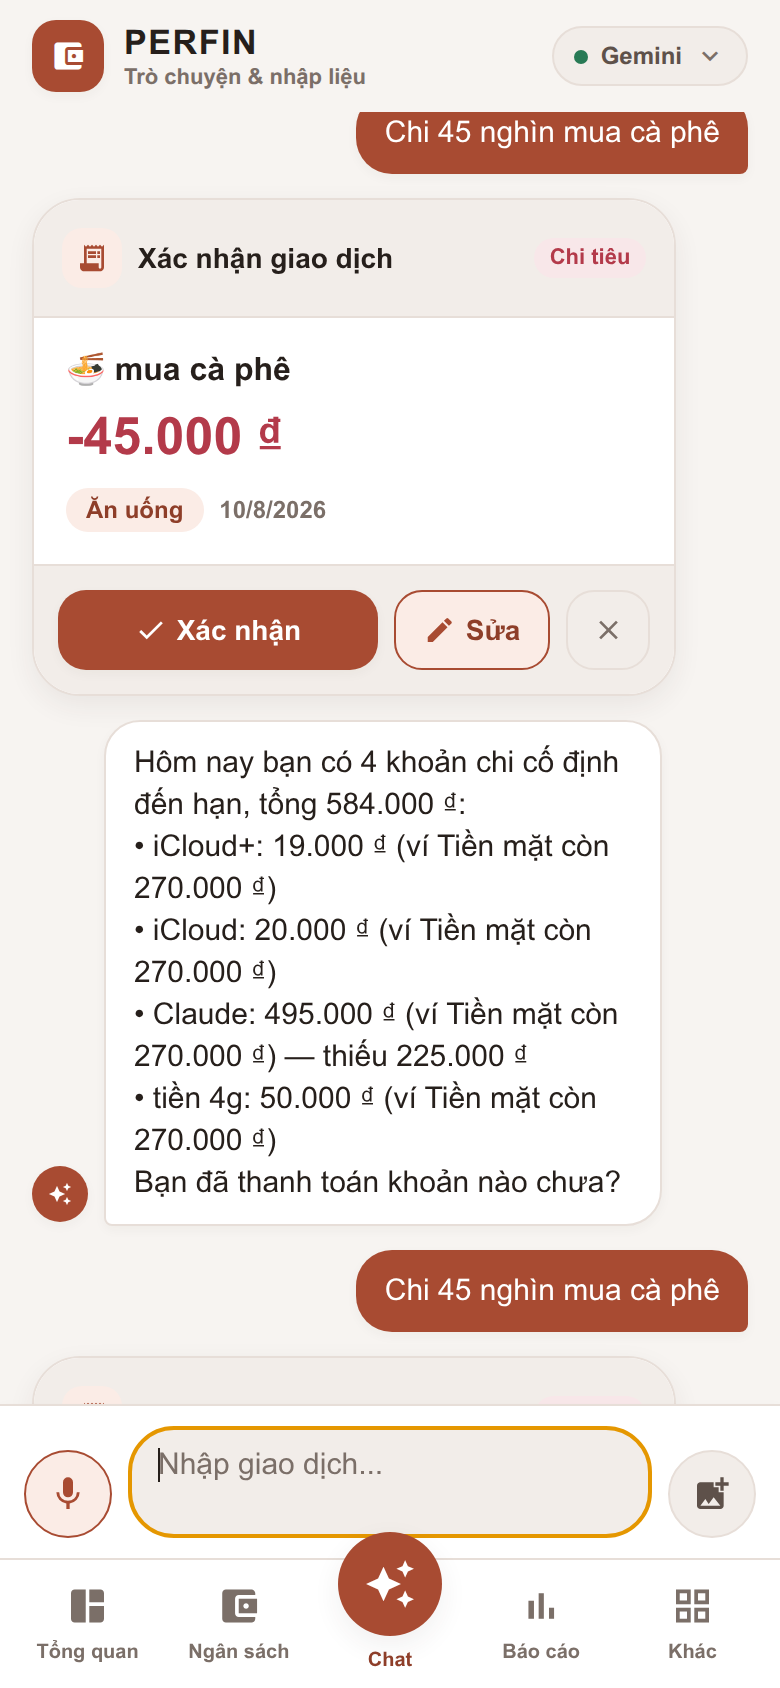
\includegraphics[width=\linewidth,height=0.48\textheight,keepaspectratio]{figures/screenshots/02-chat-preview.png}
  \end{minipage}\hfill
  \begin{minipage}[t]{0.47\textwidth}
    \centering
    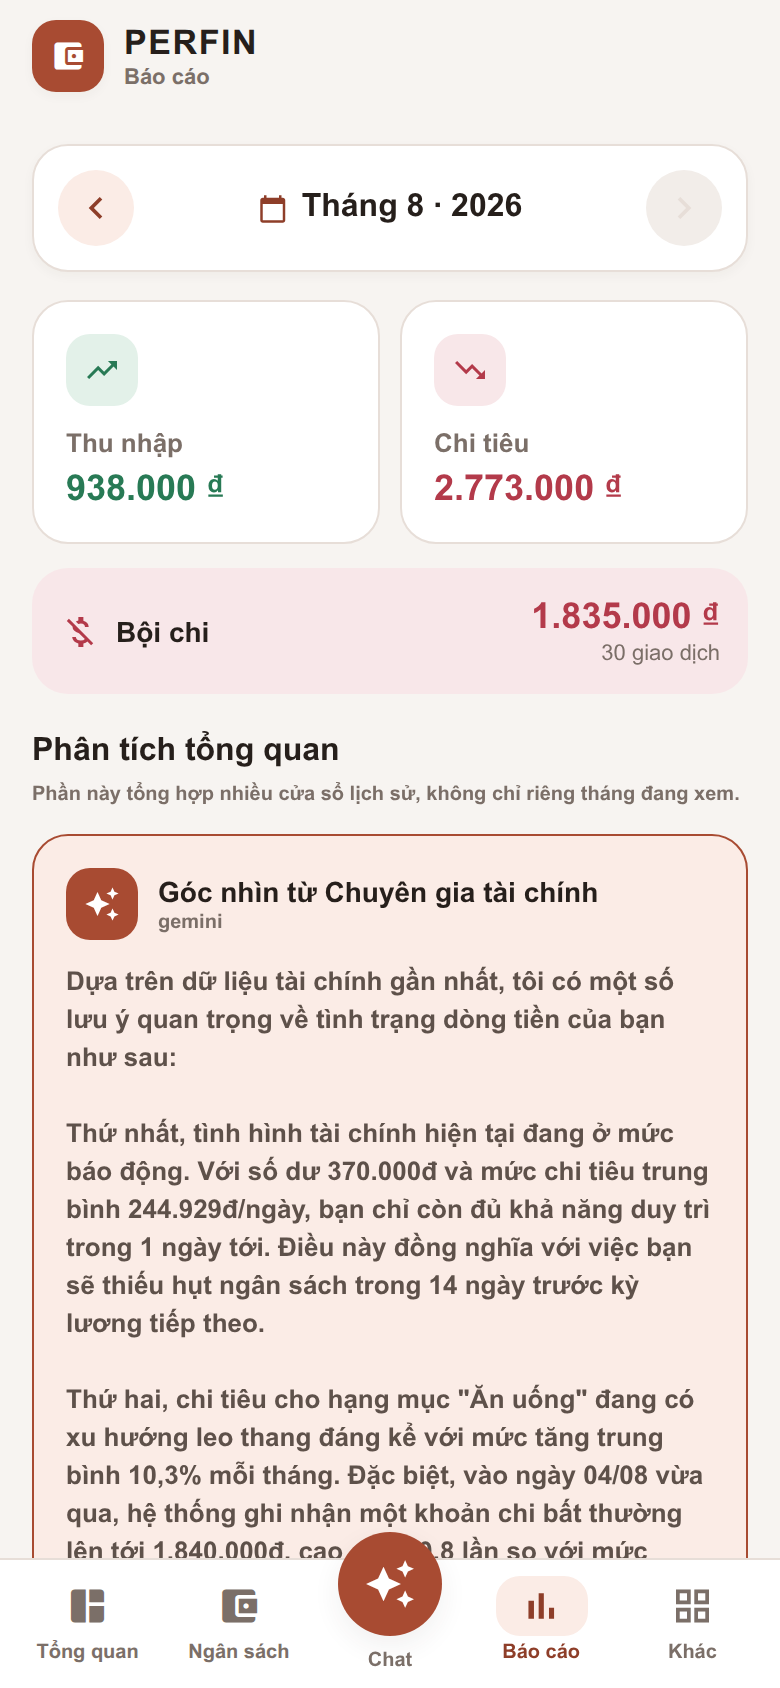
\includegraphics[width=\linewidth,height=0.48\textheight,keepaspectratio]{figures/screenshots/04-report.png}
  \end{minipage}
  \caption{Expo web mobile viewport: typed Chat preview before confirmation and loaded Report screen (synthetic data; not UAT).}
  \label{fig:ui-chat-report}
\end{figure}

\section{Software Design}

\subsection{Architecture}

PERFIN is a modular monolith: domain services are separated by responsibility while the API remains one process; a separate worker handles background jobs. This matches project scale, reduces operating cost and preserves independent module tests.

\widereportfigure{02-runtime-architecture.pdf}{PERFIN runtime architecture; the deterministic core creates and stores facts while the AI Orchestrator coordinates semantics.}{fig:runtime-architecture}

\begin{table}[H]
  \centering
  \caption{Architectural components and responsibilities}
  \label{tab:components}
  \begin{tabularx}{\textwidth}{@{}L{3.2cm}Y Y@{}}
    \toprule
    \textbf{Component} & \textbf{Responsible for} & \textbf{Not responsible for} \\
    \midrule
    Mobile App & Capture input, show previews/facts and confirm. & Database access or AI secrets. \\
    Express Routes & HTTP contracts, upload and input validation. & Analytical formulas. \\
    Core Services & Business rules, transactions and idempotency. & LLM-generated numbers. \\
    Analytics, Budget, Goal & Deterministic facts and plans. & Arbitrary advice. \\
    AI Orchestrator & Tool routing, extraction, narration and fallback. & Direct database writes. \\
    PostgreSQL & System of record, constraints and aggregates. & Temporary conversation state. \\
    Redis/BullMQ & TTL state, cache, queue and retry. & Financial source of truth. \\
    \bottomrule
  \end{tabularx}
\end{table}

Microservices were considered but not selected because prototype scale does not justify deployment, tracing and distributed-consistency costs. Serverless is also a poor fit for a long-running worker and local media providers. A modular monolith keeps database transactions simple and leaves a future extraction path when real load evidence exists.

\subsection{Data Design}

\widereportfigure{04-domain-class.pdf}{PERFIN UML domain class model separating ledger, planning, recurring and conversation/feedback aggregates.}{fig:domain-class}

\code{User} is the ownership root; \code{Wallet}, \code{Transaction} and \code{Category} form the ledger; \code{Budget}, \code{FinancialGoal} and recurring classes form planning; \code{ChatMessage} and \code{AIFeedback} preserve traceable interaction. Engines are not entities because they only read data and create facts.

\widereportfigure{05-physical-erd.pdf}{Physical ERD reconciled with runtime migrations; principal business foreign keys use separate orthogonal corridors.}{fig:physical-erd}

\begin{longtable}{@{}L{4.5cm}L{3.0cm}L{6.0cm}@{}}
  \caption{Entities in alphabetical order}\label{tab:data-entities}\\
  \toprule
  \textbf{Entity} & \textbf{Type} & \textbf{Description} \\
  \midrule
  \endfirsthead
  \toprule
  \textbf{Entity} & \textbf{Type} & \textbf{Description} \\
  \midrule
  \endhead
  \code{ai_feedback_logs} & History & Original AI result, correction and context. \\
  \code{ai_personalities} & Catalogue & Selectable persona and style prompt. \\
  \code{backup_config} & Configuration & Per-user backup policy; worker backup is not proven. \\
  \code{budget_history} & History & Audit trail of budget-limit changes. \\
  \code{budgets} & Planning & Category and monthly limits. \\
  \code{categories} & Catalogue & Income/expense taxonomy and parent relation. \\
  \code{chat_messages} & History & Conversation, facts/metadata and event key. \\
  \code{export_history} & Operations & Exported files, filters and expiry. \\
  \code{financial_goals} & Planning & Goal, progress, deadline and linked wallet. \\
  \code{investment_pnl} & Ledger & Realized investment gain/loss. \\
  \path{recurring_bill_payments} & Ledger & Payment record for each recurring period. \\
  \code{recurring_bills} & Planning & Amount, frequency and next due date. \\
  \path{recurring_suggestions_dismissed} & History & Signature of a dismissed recurring suggestion. \\
  \code{transactions} & Ledger & Income/expense, input source and soft-delete status. \\
  \code{user_traits} & Personalization & Consent-dependent user traits. \\
  \code{users} & Data root & Demo profile and data-scope key. \\
  \code{wallet_transfers} & Ledger & Transfer between two wallets. \\
  \code{wallets} & Ledger & Wallet balance, type and name. \\
  \bottomrule
\end{longtable}

Money uses \code{DECIMAL(15,2)}; report queries exclude soft-deleted records; deleting a referenced category is blocked or controlled by re-tagging; pending state exists only in Redis; and target-design ID queries include \code{user_id/user_key}. Internal transfer requires matching wallet currencies. Runway sums only liquid VND \code{cash}, \code{bank} and \code{e_wallet} balances; foreign-currency, savings, investment and credit-card wallets are excluded because the prototype has neither exchange-rate nor liquidity modelling.

\subsection{Detailed Design}
\label{subsec:detailed-design}

\subsubsection{LLM Boundary and Input}

\widereportfigure{06-llm-boundary.pdf}{LLM responsibility boundary: typed drafts and narration remain outside validation, calculation and data-write authority.}{fig:llm-boundary}

The LLM only creates a typed command or narrates facts. The backend validates schema and domain rules, builds a preview and waits for confirmation before opening a transaction. For analysis, SQL and the engine create facts before narration. A parser or deterministic template provides a testable fallback.

\widereportfigure{08-text-sequence.pdf}{Text-entry sequence; the data-write transaction starts only after confirmation.}{fig:text-sequence}

Parsing/preview has no side effect; confirm/commit atomically claims pending state. State contains intent, missing fields, candidates and a draft with a five-minute TTL. Concurrent confirmation must not create two transactions from one \code{pending_id}.

\widereportfigure{09-multimodal-flow.pdf}{Image and speech processing; both branches converge on the text pipeline after raw-text review.}{fig:multimodal-flow}

OCR/STT returns only raw text and provider metadata. Current ground truth is too small and receipt line totals are not automatically reconciled, so Figure~\ref{fig:multimodal-flow} is a design flow, not evidence of accuracy.

\subsubsection{Classification and Correction Retrieval}
\label{subsec:classification-design}

\widereportfigure{10-feedback-flow.pdf}{Classification and correction-retrieval flow; feedback is stored only after confirmation.}{fig:feedback-flow}

The matcher uses

\begin{equation}
  s=\max(s_{edit},\;0.92s_{dice},\;s_{contain}).
\end{equation}

Let $U,V$ be normalized token sets and choose $|U|\leq|V|$. The implementation defines containment as

\begin{equation}
  s_{contain}=\begin{cases}
    \min\!\left(0.94,\;0.82+0.12\dfrac{|U|}{|V|}\right),
      & U\subseteq V\ \text{and}\ |U|\geq2,\\
    0, & \text{otherwise}.
  \end{cases}
\end{equation}

Selection proceeds through exact name, exact alias and fuzzy matching. Input length is measured after normalization: input longer than four characters uses $\tau=0.82$, shorter input uses $\tau=0.90$, and the best candidate must exceed the second by $m=0.08$. These are prototype starting values, not universal optima. Retrieval loads at most 200 recent corrections and overrides only with a record of the same income/expense type; legacy records without type are ineligible. A fuzzy correction needs at least 0.88 similarity, and competing labels require at least 0.8 agreement for the winner. Multiple labels for one exact text return fallback/clarification instead of majority voting.

\subsubsection{Analytics and Planning Algorithms}
\label{subsec:analytics-design}

Default windows are 14 calendar days for runway, 30 calendar days for anomaly, 200 days for recurring discovery, six completed months for trend, 60 calendar days for day-of-week analysis and 12 completed ISO weeks for correlation. Fixed day/month/week axes zero-fill inactive periods; an incomplete current month/week is excluded from comparisons. A payday is a local day-of-month and day 31 is clamped to the target month's last calendar day.

Runway uses only liquid VND balance:

\begin{equation}
  B=\sum_{\substack{w.currency=\mathrm{VND}\\
  w.type\in\{\mathrm{cash},\mathrm{bank},\mathrm{e\_wallet}\}}} balance_w.
\end{equation}

For daily expense $e_j$ and $W=14$,

\begin{equation}
  \bar e_W=\frac{1}{W}\sum_{j=1}^{W}e_j,\qquad
  d=\left\lfloor\frac{B}{\bar e_W}\right\rfloor.
\end{equation}

If $B\leq0$, then $d=0$; if $\bar e_W=0$, the depletion date is undefined. For monthly spending $y_j$, the trend detector keeps the zero-filled six-month axis but requires at least three positive observed months, then uses OLS and emits a signal only when slope $b>0$, $R^2\geq0.5$, and mean stepwise percentage change (over steps with a positive preceding value) is at least 10\%.

Anomaly detection uses the sample standard deviation over all 30 days. It is evaluated only when at least four calendar days have positive spending, and flags only the upper tail when

\begin{equation}
  z_i=\frac{e_i-\bar e}{s}\geq2.5
  \quad\text{or}\quad
  e_i>Q_3+1.5\,IQR.
\end{equation}

When $s=0$, the implementation sets $z_i=0$; when $IQR=0$, the IQR branch is disabled. Thus a constant series cannot become anomalous merely because the denominator is undefined.

Recurring grouping normalizes descriptions and simultaneously requires at least three occurrences, every $\delta_i=|a_i-\bar a|/\bar a\leq0.15$, and gap coefficient of variation $CV_g=\sigma_g/\bar g\leq0.12$ (population $\sigma_g$ over positive gaps). Every gap must fit one cadence: weekly 5--9 days, monthly 26--35 days or quarterly 80--100 days. A candidate is active only when its latest occurrence is no older than that cadence's maximum gap; the output also records \code{lastSeen} and the calendar-clamped \code{nextExpected}. There is no default amount ceiling. The monthly estimate is

\begin{equation}
  \widehat a_{month}=\begin{cases}
    \bar a\,52/12, & \text{weekly},\\
    \bar a, & \text{monthly},\\
    \bar a/3, & \text{quarterly}.
  \end{cases}
\end{equation}

Correlation zero-fills a shared 12-week axis, keeps categories observed in at least four weeks and skips undefined Pearson pairs (fewer than three paired observations or zero variance). It returns only the strongest positive pair when $r\geq0.6$; association does not imply causation. Day-of-week analysis uses the 60-day window, requires at least four observed weekdays and emits a signal only when the peak-to-mean ratio reaches 1.8.

For category spending $s_{c,j}$ across $m$ months, a five-percent-buffer baseline is

\begin{equation}
  b_c=1.05\left(\frac{1}{m}\sum_{j=1}^{m}s_{c,j}\right).
\end{equation}

Month-end forecast is $\widehat S_D=(S/d_e)D$, where $S$ is spending so far, $d_e$ elapsed calendar days including today and $D$ month length. The 50/30/20 and hybrid strategies shrink raw allocations when they exceed a cap; post-rounding reconciliation keeps each group at or below its cap. Needs, wants and savings rates may not sum to more than 1; recommendations require confirmation.

For a saving or purchase goal with remaining amount $R$ and monthly contribution $M>0$, $n_s=\lceil R/M\rceil$. For current debt principal $L$ and nominal annual percentage rate $i$, the implementation uses monthly rate $r=i/(12\times100)$. With a debt deadline of $n_d$ months, the required end-of-month level payment is

\begin{equation}
  P=\frac{Lr}{1-(1+r)^{-n_d}}
\end{equation}

for $r>0$, and $P=L/n_d$ for $r=0$. A payment less than or equal to first-month interest triggers a negative-amortization warning; a zero payment is reported separately. Without a deadline, the implementation simulates month by month up to a 600-month default horizon. What-if currently reruns the saving/purchase function with an additional contribution; debt plans are not changed by that scenario, and no what-if result is persisted.

\widereportfigure{12-goal-flow.pdf}{Goal planning and what-if flow; only final confirmation persists a goal.}{fig:goal-flow}

\subsubsection{Grounded Insight Generation}

\widereportfigure{11-insight-sequence.pdf}{Grounded-insight sequence; Analytics returns facts before persona/LLM narration.}{fig:insight-sequence}

Facts contract version 1.0 returns \code{schema_version}, \code{generated_at}, each component value and \code{metadata.components}. Per-component metadata contains \code{unit}, \code{window}, \code{sample_count}, \code{method}, \code{parameters}, \code{warnings}, and \code{status} in \code{ok/no_signal/degraded}. The window object records \code{size}, \code{unit} and \code{zero_filled}; selected components add \code{category_count} or \code{wallet_count}. A local failure appears in \code{degraded_components} without removing the contract. A persona changes tone only with consent; the response includes narration and facts for UI/test comparison. A numeric checker covering every expression remains a target design.

The calculation path, numeric examples and boundary cases for matching, correction, Analytics, Budget, Goal and the facts contract are expanded in Appendix~\ref{app:algorithms}--\ref{app:facts-contract}; this chapter keeps the main formulas and design decisions for a coherent core narrative.

\section{Testing}
\label{sec:testing}

\subsection{Test Plan}

\begin{longtable}{@{}L{2.2cm}L{3.7cm}L{4.2cm}L{3.9cm}@{}}
  \caption{Test-plan matrix}\label{tab:test-matrix}\\
  \toprule
  \textbf{Level} & \textbf{Target} & \textbf{Technique} & \textbf{Expected evidence} \\
  \midrule
  \endfirsthead
  \toprule
  \textbf{Level} & \textbf{Target} & \textbf{Technique} & \textbf{Expected evidence} \\
  \midrule
  \endhead
  Unit & Matching, analytics, budget, goal and validation. & Normal, boundary, hand-computed expected values and invariants. & \code{node:test} pass/fail by case. \\
  Integration & Route--service--model, PostgreSQL and Redis. & Test DB, rollback, TTL and concurrent claim. & Logs, DB snapshots and exit code. \\
  System & Text/voice/image through preview and DB. & End-to-end scripted smoke. & HTTP response, DB assertion and UI image. \\
  AI contract & Parser, tool schema, LLM and corrections. & Joint type/category labels; abstentions stay in the denominator; whole-group split. & JSON records, coverage, accuracy/F1 and helped/harmed/net. \\
  Media & OCR/STT adapters. & Ground-truth image/audio. & CER/WER and field accuracy. \\
  Worker & Retry, deduplication and schedule. & Repeated fingerprint and fault injection. & Before/after effect count. \\
  UAT & Target users. & Timed tasks and step count. & Completion, duration and SUS. \\
  \bottomrule
\end{longtable}

The text dataset must cover currency units, written numbers, multiplication, relative dates, multiple transactions, typos, mixed Vietnamese/English, missing or ambiguous fields and conflicting corrections. In correction evaluation, every row sharing transaction type and normalized description must lie wholly in seed or evaluation. Analytics data needs known slopes, outliers, cadence and correlation. Media data must store image/audio with a reference transcript or receipt table.

The normal-case, boundary-case, invariant and test-file catalog is provided in Appendix~\ref{app:algorithm-tests}; the source, schema, cohorts and dataset limitations are documented in Appendix~\ref{app:dataset-description}. These appendix tables point to evidence without replacing the measured results in Section~\ref{subsec:results}.

\subsection{Results and Analysis}
\label{subsec:results}

\subsubsection{Measured Operational Results}

\begin{longtable}{@{}L{3.4cm}L{3.5cm}L{2.4cm}L{4.4cm}@{}}
  \caption{Measured results and conclusion boundaries}\label{tab:measured-results}\\
  \toprule
  \textbf{Item} & \textbf{Result} & \textbf{Status} & \textbf{Permitted conclusion} \\
  \midrule
  \endfirsthead
  \toprule
  \textbf{Item} & \textbf{Result} & \textbf{Status} & \textbf{Permitted conclusion} \\
  \midrule
  \endhead
  Targeted regression (21 cases) & 21/21 pass for analytics, invariants and media-provider boundary tests. & \statusmeasured & Command and fixture are reproducible; this is a focused subset, not the full suite. \\
  Backend \code{npm test} & 247/247 tests pass with Redis and jobs disabled. & \statusmeasured & The backend suite passes in the current worktree; live Redis-worker behavior is not measured. \\
  Node 24 test coverage & 68.12\% line, 72.77\% branch and 72.27\% function coverage over all loaded backend files. & \statusmeasured & Instrumentation is reproducible; the planned component thresholds (line/function $\geq85\%$, branch $\geq75\%$) are not yet demonstrated. \\
  Local-parser gate and API smoke & Pending clean rerun on the current snapshot. & \statusmissing & Existing artifacts belong to an older worktree and are not current evidence. \\
  Mobile-web UI smoke & 5/5 synthetic captures pass at 390$\times$844. & \statusmeasured & Dashboard, Budget, Report, Chat preview and Goal plan loaded without overflow; Expo web only, not native-device or UAT evidence. \\
  Data profile & 5,328 source rows, 0 validation errors; SHA prefix \code{418a...}. & \statusmeasured & Dry-run profile covers 01 Jan 2022--10 Aug 2026; PostgreSQL apply is a separate step. \\
  Current experiments & Rerun pending on the 5,328-row snapshot. & \statusmissing & Primary metric is joint type/category; correction must reproduce the production candidate limit of 200. \\
  Parser versus Gemini ablation & Rerun pending with joint labels and complete sample-level records. & \statusmissing & Category-only scores may be auxiliary; abstentions remain in the denominator. \\
  OCR/STT accuracy & Pending 20-image and 20-audio ground truth. & \statusmissing & CER/WER and transaction-field accuracy cannot be inferred from smoke execution. \\
  Live Redis worker, grounding, p95 and UAT & Pending controlled environment and target participants. & \statusmissing & Requires duplicate-effect assertions, a checker, at least 30 timed runs per flow and five or more users. \\
  \bottomrule
\end{longtable}

Smoke testing only establishes completion of selected scenarios. It is not OCR/STT accuracy evidence, and a tested payment handler does not prove that a live Redis worker ran.

\subsubsection{Classification Experiments}

The current source is \code{demo/data/dataFinance.csv}, profiled at 5,328 rows with SHA-256 prefix \code{418a9439...fbaed7}. The classification, Gemini ablation and correction artifacts that used the previous 5,265-row file are retained for audit but are superseded and are not reported as current measurements.

The rerun protocol is fixed before new data is supplied:

\begin{table}[H]
  \centering
  \caption{Classification and correction rerun protocol}
  \label{tab:exp-classification}
  \begin{tabularx}{\textwidth}{@{}L{3.0cm}Y Y@{}}
    \toprule
    \textbf{Experiment} & \textbf{Primary measurement} & \textbf{Required evidence} \\
    \midrule
    Local parser & Joint type/category accuracy, macro-F1, weighted-F1 and per-class support; category-only is auxiliary. & Current CSV hash, complete record-level predictions and deterministic command. \\
    Parser--Gemini ablation & Joint-label coverage, full-set accuracy/F1, answered metrics and latency; abstentions remain in the denominator. & Repeated sample-level records, model/configuration and provider error count. \\
    Correction retrieval & Before/after joint label, coverage and helped/harmed/net under a chronological group split. & Candidate limit 200, no future rows in retrieval, seed/evaluation key overlap zero and confidence interval. \\
    \bottomrule
  \end{tabularx}
\end{table}

The correction runner now records the production-equivalent candidate limit of 200 and exposes the candidate count per row. Its current ordering uses source-row order as a documented chronological proxy; a future dataset with trustworthy timestamps should replace that proxy with an explicit temporal replay. The ablation runner now makes the joint type/category label primary and keeps category-only metrics only as an auxiliary view.

\begin{table}[H]
  \centering
  \caption{Status of experiment artifacts on the current snapshot}
  \label{tab:exp-ablation}
  \begin{tabularx}{\textwidth}{@{}L{4.0cm}L{3.0cm}Y@{}}
    \toprule
    \textbf{Artifact} & \textbf{Status} & \textbf{Reason for withholding a score} \\
    \midrule
    Local classification & \statusmissing & The old artifact used a different CSV and must be regenerated. \\
    Parser--Gemini ablation & \statusmissing & The old record lacks complete joint-label predictions; rerun requires provider access and quota. \\
    Correction retrieval & \statusmissing & The old runner exposed all seed logs rather than the production 200-candidate window. \\
    \bottomrule
  \end{tabularx}
\end{table}

These statuses preserve traceability without treating a historical experiment as a claim about the current code or dataset. Once the user supplies controlled fixtures, the resulting JSON and Markdown artifacts can be inserted without changing the metric definitions.

\subsection{Requirements-to-Evidence Traceability}

Table~\ref{tab:traceability} links observable requirements to design, tests and evidence status. A route, mock or diagram alone is not end-to-end acceptance evidence.

\begin{longtable}{@{}L{2.2cm}L{3.4cm}L{3.5cm}L{4.8cm}@{}}
  \caption{FR--design--test--evidence traceability}\label{tab:traceability}\\
  \toprule
  \textbf{Req.} & \textbf{Design} & \textbf{Related test} & \textbf{Evidence and gap} \\
  \midrule
  \endfirsthead
  \toprule
  \textbf{Req.} & \textbf{Design} & \textbf{Related test} & \textbf{Evidence and gap} \\
  \midrule
  \endhead
  FR-01, FR-03--FR-05 & Typed draft, TTL preview, service and SQL transaction. & Parser gate, backend tests and API--DB smoke. & Selected fixtures and rollback invariants pass; no independent task-based user measurement. FR-06 is specified in the appendix. \\
  FR-02 & Media adapter, raw-text review and shared FR-01 pipeline. & Upload/media smoke; planned CER/WER and field accuracy. & Sample provider flow executes; insufficient ground truth for OCR/STT accuracy. \\
  FR-04 & Joint classifier, type-scoped corrections, conflict thresholds and group split. & Classification benchmark, ablation coverage and correction helped/harmed/net. & Rerun is pending on the current CSV and production candidate window; historical scores are superseded. \\
  FR-07--FR-10 & Analytics, facts contract, Budget/Goal service and grounded narrator. & Hand-expected unit tests, metadata contract and planned checker. & Formulas, calendar windows and metadata have tests; response-wide grounding and representative threshold calibration remain incomplete. \\
  FR-11 & Recurring service, BullMQ, event key and retry. & Payment/handler unit tests; planned live worker and fault injection. & Business logic is tested; no live queue/worker evidence in this evaluation. \\
  FR-12 & CSV exporter, history and TTL cleanup. & Escaping tests, API smoke and planned expiry check. & CSV has evidence; the former PDF-labelled path only generates HTML. \\
  NFR-01--NFR-08 & Constraints, user scope, fallback, idempotency and fact metadata. & Rollback, cross-scope, load, recovery, worker and UAT. & Test integrity has evidence; three-hour recovery, p95, UAT, live worker and faithfulness remain targets. \\
  \bottomrule
\end{longtable}

\subsection{Threats to Validity}

\subsubsection{Internal Validity}

Benchmarks depend on historical labels, and identical descriptions may have different categories. The new correction experiment splits whole type+normalized-description groups with zero overlap, but seed and evaluation still come from one dataset, use one seed and have no confidence interval. The 63-sentence ablation is small; its historical artifact omitted complete prediction records and computed conditional metrics after removing 21 abstentions, so full-set Gemini macro-F1 cannot be recovered. Providers also vary by version and time; the updated runner therefore stores model, parameters, timestamp and sanitized structured records.

\subsubsection{Construct Validity}

The 31/31 gate measures success on designed sentences, not out-of-sample correctness. Smoke tests measure scenario completion, not accuracy or usability. Accuracy can hide rare classes, while abstention can inflate conditional metrics. Coverage, macro-F1, weighted-F1, per-class confusion, helped/harmed/net and support are therefore reported together. For OCR/STT, CER/WER alone is insufficient: amount, date and merchant field accuracy maps more directly to ledger risk.

\subsubsection{External Validity}

Data comes from one demo profile, uses VND and is primarily Vietnamese. Results do not automatically generalize to many users, other taxonomies, varied receipts or production load. The next evaluation should lock the taxonomy, sample randomly over time, retain group splitting while running multiple seeds/confidence intervals, and add target-user UAT. Conclusions apply only to the source, dataset and environment recorded in the 24 July ablation and 2 August 2026 classification/correction artifacts.
